\documentclass[a4paper, 12pt]{article}
\usepackage[english,russian]{babel}
\usepackage{amsfonts}
\usepackage{pgfplots}
\usepackage[utf8]{inputenc}
\usepackage{amsmath,amssymb}

\begin{document}
	\begin{Huge}
		\begin{center}
			\textbf{Отчет о выполнении лабораторной работы 2.3.1}\\
			\vspace{2em}
			\textbf{Получение и измерение вакуума при турбомолекулярной
				откачке}\\
			\vspace{5em}
			\textbf{Выполнил: }Тимонин Андрей\\
			\textbf{Группа: }Б01-208\\
			\vspace{10em}
			\textbf{Дата: }22.03.2023\\
		\end{center}
	\end{Huge}

\section{Введение}
\noindent\textbf{Цель работы:} 1) измерение объемов форвакуумной и высоковакуумной частей установки; 2) определение скорости откачки системы в стационарном режиме, ухудшениe и улучшение вакуума.\\
\bigskip

\noindent\textbf{В работе используются:} вакуумная установка с манометрами: масляным, термопарным и ионизационным.
\section{Экспериментальная установка}
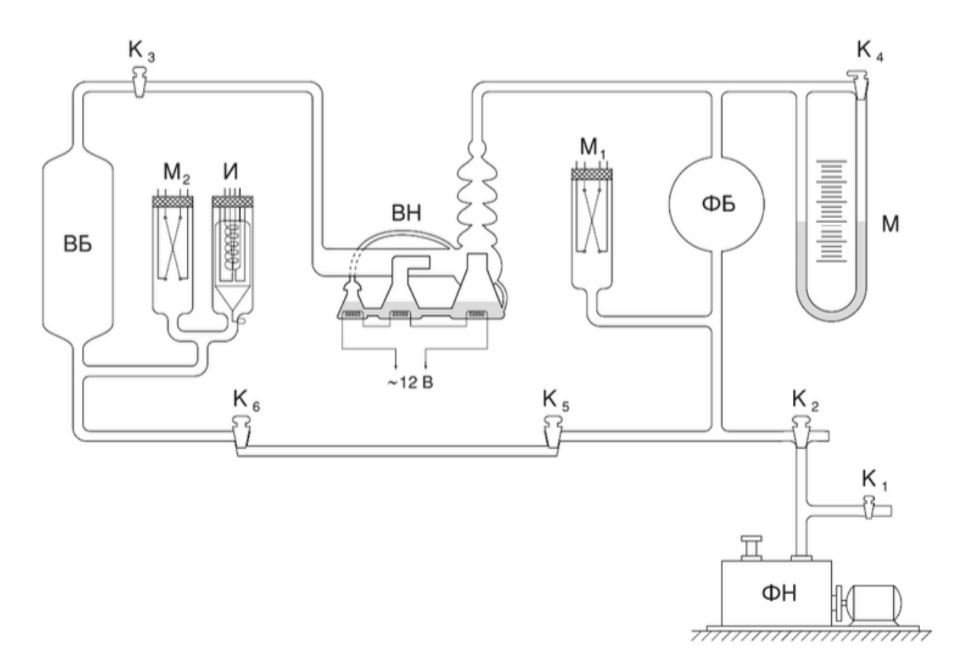
\includegraphics[width=15cm]{11.jpg}
\begin{center}
	Рис. 1 Схема экспериментальной установки
\end{center}
Установка изготовлена из стекла,
и состоит из форвакуумного баллона (ФБ), высоковакуумного диффузионного насоса (ВН), высоковакуумного баллона (ВБ), масляного (М) и ионизационного (И) манометров, термопарных манометров ($M_1$ и $M_2$), форвакуумного насоса (ФН) и соединительных кранов ($K_1, K_2,\; \ldots \;K_6$) (Рис. 1). Кроме того, в состав установки входят: реостат и амперметр для регулирования тока нагревателя диффузионного насоса.\\

\begin{center}
	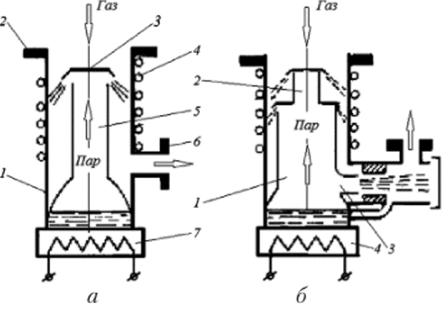
\includegraphics[width=14cm]{2.jpg}
	Рис. 2 Устройство диффузионного насоса (в лабораторной установке используется несколько откачивающих ступеней)
\end{center}
Принцип работы диффузионного насоса описан ниже: \\ 
 Масло, налитое в сосуд, подогревается электрической печкой. Пары масла поднимаются по трубе и вырываются из сопла. Струя паров увлекает молекулы газа, которые поступают из откачиваемого сосуда через трубку. Дальше смесь попадает в вертикальную трубу. Здесь масло осаждается на стенках трубы и маслосборников после чего стекает вниз, а оставшийся газ откачивается форвакуумным насосом.

\section{Экспериментальные данные}
\subsection{Определение объемов форвакуумной и высоковакуумной частей установки}
\textbf{Дано:}\\
1)Атмосферное давление 742.9 мм. рт. ст. ($P_{atm} = 99.04$ кПа)\\
2)V = 50 $cm^3$ - объём «запертого» в сильфоне воздуха\\
3)$P_1 = 2.5 \cdot 10^{-2}$ мм. рт. ст\\
4)Плотность масла: 8.85 $\frac{g}{{cm}^3}$\\
\bigskip 5)Плотность ртути: 13.6 $\frac{g}{{cm}^3}$

\begin{enumerate}	
\item \textbf{Проверим все краны установки.}
\item \textbf{Откроем краны и запустим воздух в установку(подождем 5 минут пока воздух заполнит установку).}
\item \textbf{Запрем объем воздуха V и включим форвакуумный насос.}	
\item \textbf{Отсоединим установку от насоса и откроем кран сифона.}
\item \textbf{Запишем показания масляного манометра.}\\ 

\noindent$h_1 = (38 \pm 0.1)$ см. масляного столба\\
$h_2 = (12 \pm 0.1)$ см. масляного столба\\
$\bigtriangleup h_{1-2} = 26$ см масляного столба \\
\bigskip $P_{1-2} =  225.78 $ кПа\\

\item \textbf{Откроем кран, который соединяет установку с высоковакуумной частью и запишем данные.}\\ 

\noindent$h_3 = (34 \pm 0.1)$ см. масляного столба\\
$h_4 = (17.0 \pm 0.1) $ см. масляного столба\\
$\bigtriangleup h_{3-4} = 17$ см масляного столба \\
$P_{3-4} =  147.6 $ кПа\\

\begin{align}
	\sigma_{\Delta h_{1-2}} = \sqrt{\sigma_{h1}^2 + \sigma_{h2}^2}\approx 0.6~\% & &
	\Delta h_{1-2} = (26.0 \pm 0.2)  cm
\end{align}

\begin{align}
	\sigma_{\Delta h_{3-4}} = \sqrt{\sigma_{h3}^2 + \sigma_{h4}^2}\approx 0.7~\% & &
	\Delta h_{3-4} = (17.0 \pm 0.1)  cm
\end{align}\bigskip

\item \textbf{Вычислим объем форвакуумной части установки}\\ 
\begin{align}
	V_{forv} = \frac{13.6 \cdot 742.9}{0.885\cdot 26 \cdot 10} \cdot 50 = 2195.0 cm^3
\end{align}

Отсюда получаем приблизительную погрешность определения  объема форвакуумной части установки:
\begin{align}
	\varepsilon_{V_{total}} = \varepsilon_{\Delta h_{1-2}} \approx 1~\%
\end{align}

\item \textbf{Вычислим объем высоковакуумной части установки}\\ 
\begin{align}
	V_{vis-vac} = \frac{P_{atm}\cdot V}{P_{3-4}} - V_{forv} = \frac{13.6 \cdot 742.9 \cdot 50}{170 \cdot 0.885} -  2195.0 =  1162.0 cm^3
\end{align}

Отсюда получаем приблизительную погрешность определения полного объема установки:
\begin{align}
		\varepsilon_{V_{total}} = \varepsilon_{\Delta h_{3-4}} \approx 1~\%
\end{align}

Найдем погрешность определения объема высоковакуумной части установки:
\begin{align}
	\sigma V_{vis-vac} = \sqrt{\sigma^2 V_{total} + \sigma^2 V_{frov}} = 0.01
\end{align}
	
\end{enumerate}

\subsection{Получение высокого вакуума и измерение скорости откачки}

$P_{pred} = 4.0 \cdot 10^{-5}$\\ мм. рт. ст

ВИТ 16 $P = 3 \cdot 10^{-4}$ мм. рт. ст.
$U = 9.93 mB$

Построим график зависимости $ln(P-P_0)$ от времени \\

\begin{center}
	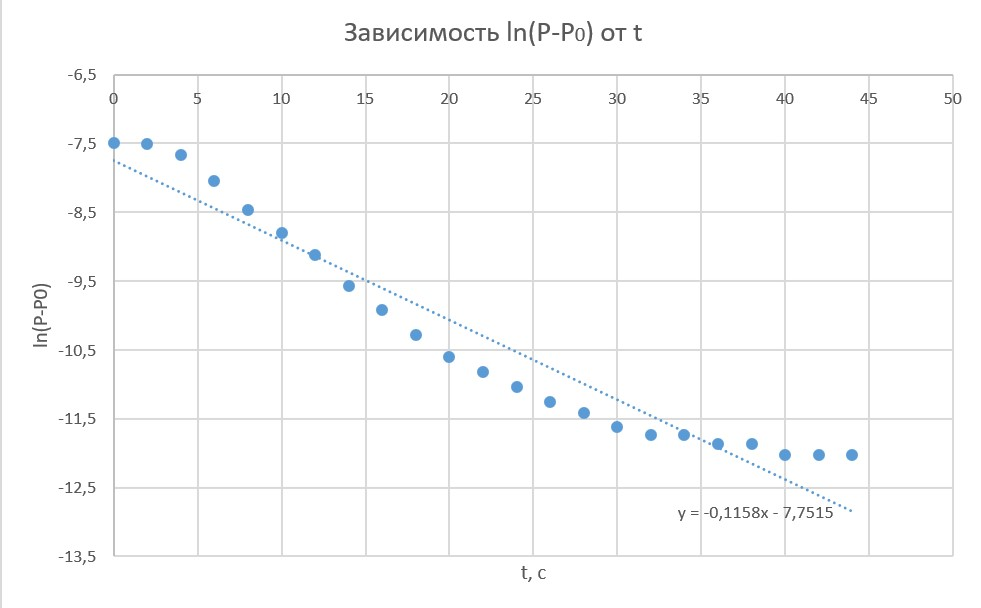
\includegraphics[width=15cm]{13.jpg}
	Рис 3. Улучшение вакуума
\end{center}

Для случая улучшения вакуума построим график зависимости $(ln(P-P_{pred}))$ от $t$. При построении такого графика из МНК получим коэффициент наклона --- $k$, с помощью которого можно найти $W = -kV_{vis-vac}$. (объем газа, \bigskip удаляемого из сосуда при данном давлении при единицу времени)\\

Оценим величину потока газа  $Q_h$ (обратный ток через насос) используя данные при ухудшении вакуума. Построим график зависимости $P(t)$. Поскольку $V_{vis-vac}dP = (Q_d + Q_i) dt$ получим $(Q_d + Q_i) = kV_{vis-vac}$.
\begin{center}
	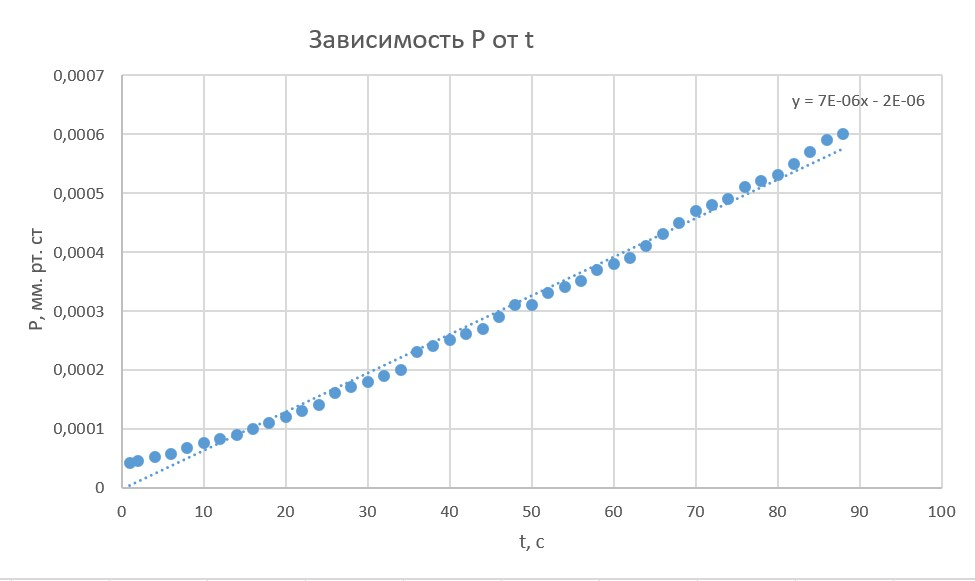
\includegraphics[width=15cm]{12.jpg}\\
	Рис 4. Ухудшение вакуума
\end{center}

\textbf{Имеем:}
\begin{align}
	W = -0.12 \cdot 1162.0 = - 139.4 \frac{cm^3}{s} = -0.1394 \frac{l}{s}
\end{align}
и
\begin{align}
	Q_h = W \cdot P_{pred} - k \cdot V_{vis-vac} = -0.000139 \cdot 4 \cdot 10^{-8}\cdot 9.81 \\ \cdot 13800 - 7 \cdot 10^{-6} \cdot 0.001162 = - 7.4 \cdot 10^{-7} \frac{kg \cdot m^3}{s}
\end{align}

\section{Вывод}
\begin{itemize}
	\item Нашли объемы форвакуумной и высоковакуумной установки, так же как и общий объем установки($V_{forv} = 2195.0 \pm 22.0 cm^3, V_{vis-vac} = 1162.0 \pm 16.5 cm^3, V_{total} = 3407.0 \pm 34.1 cm^3$).
	\item Определили скорость откачки ($- 139.4 \frac{cm^3}{s}$).
	\item Сделали оценку потока газа, который поступает из нашего насоса в откачиваемую систему установки ($- 7.4 \cdot 10^{-7} \frac{kg \cdot m^3}{s}$).
\end{itemize}

\end{document}